%%
%
% TODO:
% - talk somewhere about the types of attack which we allow
% - make sure I talk about the types of channel which we use
% Q: where should I talk about Alice's function F?
% - understand the mapping from complex values to binary
% - some more remarks about the running of the protocol?
% - mention somewhere my linestyle convention for different types of channel

\chapter{Quantum secret sharing}\label{chapter:qss}


In this chapter we introduce and investigate a continuous-variable Quantum Secret Sharing (QSS) protocol, which allows for secure distribution of a classical secret among multiple potentially dishonest recipients. Crucially, recipients are forced to collaborate in order to reconstruct the secret, and a dishonest player should not be able to access the secret by themselves.

We describe the protocol and its similarities and differences to recent QSS protocols from the literature in Sec.~\ref{sec:qss_our_protocol}, and then prove its security against several different attack strategies in Secs.~\ref{sec:qss_honest_recipients},~\ref{sec:qss_dishonest_recipient}. In Sec.~\ref{sec:qss_performance} we analyse the performance of our protocol. Although the QSS task has been around for many years, many of the existing protocols are not suitable for implementation, despite their high level of security. We present the implementation of our protocol in Chapter~\ref{chapter:aqc}.

\section{Our QSS protocol}\label{sec:qss_our_protocol}

Our Quantum Secret Sharing (QSS) scheme allows for Alice to distribute a classical secret between two recipients, Bob and Charlie. To keep with convention we call Alice the ``dealer''. Either Bob or Charlie is dishonest, and Alice does not know which one. Bob and Charlie should be able to exactly reconstruct the secret when they work together, while the dishonest player should not be able to access the secret by themselves, or even if they work with an external Eve.


\begin{figure}[htp]
\captionsetup{width=0.8\linewidth}
\centering
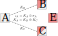
\includegraphics[draft=false, width=0.8\linewidth]{qss/qss_setup_cartoon}
\caption{\label{fig:qss_structure} All quantum secret sharing schemes follow the same structure: Alice encrypts her classical secret $\sigma_A$ with secret key $K_A$, and broadcasts the resulting $\varsigma_A$. Shares of $K_A$ are distributed among recipients Bob and Charlie such that $K_B \oplus K_C = K_A$. Gray boxes denote honest players, while red denotes dishonest players. The half-red/half-gray boxes denote uncertainty about the honesty of a player. %say somewhere it's all classical?
}
\end{figure}

\subsection{QSS setup}

All QSS protocols follow essentially the same structure, Fig.~\ref{fig:qss_structure}:
\begin{enumerate}
\item Alice (A) uses quantum resources to distribute shares of classical key $K_A$ among recipients Bob (B) and Charlie (C). These shares are labelled $K_B, K_C$ and are such that $K_A = K_B \oplus K_C$.
\item Alice encrypts her secret $\varsigma_A = K_A \oplus \sigma_A$ and makes the encrypted secret $\varsigma_A$ publicly known.
\end{enumerate}
The $\oplus$ operation corresponds to bitwise addition (XOR) of binary strings. Provided that $K_A, K_B, K_C$ and $\sigma_A$ are the same length, the above secret sharing operation is provably unconditionally secure\footnote{Much like the One Time Pad} provided that key shares $K_B, K_C$ are securely distributed \cite{Schneier1996}.

This form of protocol is similar to QKD-based encryption and it is for this reason that renowned cryptographer Gustavus Simmons wrote that 

\begin{center}\emph{``Secret sharing is simply a special form of key distribution''}\end{center}

\noindent as his abstract to Ref.~\cite{Simmons1990a}.

QSS protocols, then, only differ in the method used to generate and share the $K_B, K_C$ forming the encryption key. One potentially attractive option would be for Alice to perform individual QKD protocols, first with Bob and then with Charlie, and then XOR the resulting secure keys together. Since QKD is provably secure against a quantum adversary, neither Bob nor Charlie can gain sufficient information about the other player's key, and the resulting QSS scheme is thus also secure. Alternatively, once the secure keys are shared between Alice-Bob and Alice-Charlie, they could implement one of several classical unconditionally secure schemes which are discussed in Sec.~\ref{sec:qss_lit_review}.

Other options for distribution of a secret using quantum resources are discussed in Sec.~\ref{sec:qss_lit_review} and fall into one of two categories. The first category \cite{Hillery1999, Karlsson1999, Gottesman1999, Markham2008, Wu2016, Kogias2017} relies on large entangled states shared between all $N$ players, while the second category \cite{Zhang2005a, Schmid2005, Schmid2007, Grice2019}, involves distribution of a single (typically one-mode) quantum state between all $N$ players, who each perform their choice of measurement on the state. In both forms, if $N-1$ players communicate and share their choice of measurement and their measurement outcomes, they have sufficient information to infer the measurement outcome of the $N^{\text{th}}$ player. In this way, a key $K_A$ is distributed between players.


\subsection{QSS protocol description}

We here propose a QSS protocol which will perform the task of quantum secret sharing without requiring the distribution of highly entangled states between players \cite{Kogias2017} and without requiring a dedicated hardware or network setup \cite{Grice2019}. Instead, we rely on distribution of QPSK alphabet Eq.~\ref{eqn:intro_qpsk}, Fig.~\ref{fig:qpsk} and heterodyne detection Sec.~\ref{eqn:intro_heterodyne}. Our QSS protocol guards against eavesdropping by choosing a QPSK alphabet with small coherent state amplitude $\alpha$. This ensures that Eve cannot accurately guess Alice's heterodyne outcomes. The protocol also guards against the internal dishonesty of Bob or Charlie by ensuring that the key $K_A$, which Alice will use to encrypt her secret, is a function of \emph{both} Bob and Charlie's information.

In our protocol, Bob and Charlie are chosen as the senders of the quantum states. This has advantage in that we may fully trust Alice's heterodyne detection\footnote{Note that permitting Bob or Charlie to perform the heterodyne detection implicitly places trust in their heterodyning beamsplitter \cite{Walk2016a}. %TODO: make sure that I can talk about this for the viva
} and its characterisation. A dishonest internal player will be forced to collaborate with Eve to attack the honest player's quantum channel, but by our choice of alphabet, this will not succeed. Since Alice will decide on the eventual shared key our protocol is analogous to a reverse-reconciliation (RR) QKD system, and so we may similarly expect the performance benefits of RR QKD at high loss. Indeed, we may interpret the entire QSS protocol as effectively a QKD protocol between Alice (dealer) and several recipient players.

\begin{figure}[htp]
\captionsetup{width=0.8\linewidth}
\centering
	\begin{subfigure}{0.8\linewidth}
		\centering
		\label{fig:qss_distribution_stage}
		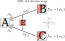
\includegraphics[draft=false, width=\linewidth]{qss/qss_distribution_stage}
	\end{subfigure}
%	\vspace{3cm}%
	\begin{subfigure}{0.8\linewidth}
		\centering
		\label{fig:qss_encryption_stage}
		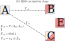
\includegraphics[draft=false, width=\linewidth]{qss/qss_encryption_stage}
		
	\end{subfigure}
\caption{\label{fig:qss_protocol_cartoon} Distribution and Encryption stages of our QSS protocol. Alice (A) wishes to securely share her secret $\sigma_A$ amongst potentially dishonest recipients Bob (B) and Charlie (C). (a) Distribution stage. B and C send coherent states chosen from QPSK alphabet to Alice, who heterodynes and obtains outcomes $A_B, A_C$. Eve eavesdrops on the quantum channels in order to gain information about Alice's outcomes $A_B, A_C$. (b) Encryption stage. Alice forms variable $X_A$ using her chosen function $\mathcal{F}$ with her heterodyne measurement outcomes as input variables. She converts $X_A$ to a binary $\tilde{X}_A$ and encrypts the secret with it to reach $\varsigma_A = \sigma_A \oplus \tilde{X}_A$. The encrypted secret is then broadcast. Dishonest players are shown in red and honest players in gray. A combination of red and gray denotes uncertainty about the honesty of a player.
}
\end{figure}


Our QSS protocol runs in three stages, a Distribution stage, an Encryption stage and, finally, a Decryption stage. Distribution and Encryption stages are displayed in Fig.~\ref{fig:qss_protocol_cartoon}. The Distribution stage, Fig.~\ref{fig:qss_distribution_stage}, involves distribution and measurement of quantum coherent states chosen from QPSK alphabet. At the end of Distribution, Alice will hold classical information which is correlated with both Bob and Charlie. In the Encryption stage, Fig.~\ref{fig:qss_encryption_stage}, Alice will combine her classical information and use it to encode her sensitive classical secret. The encoded secret is then distributed to Bob and Charlie, who decode it during Decryption. 


\subsubsection*{Distribution stage, Fig.~\ref{fig:qss_protocol_cartoon}a}
\paragraph{Step $1$}
Alice wishes to share a classical secret, $\sigma_A$. Bob forms a classical random variable $X_B = \left\{\phi_B\right\}$, where the $\phi_B$ are one of four complex phases independently chosen from the QPSK alphabet. Phases $\phi_B$ are assumed to be chosen uniformly at random, but we relax this assumption in Chapter~\ref{chapter:aqc}. Charlie likewise forms classical random variable $X_C = \left\{\phi_C\right\}$.

\paragraph{Step $2$}
Bob and Charlie form sequences of coherent states based on their random variables
\begin{equation}
\rho\left[X_{\left(B, C\right)}\right] := \otimes \rho\left[\phi_{\left(B, C\right)}\right]
\end{equation}
where $\rho\left[\phi_{\left(B, C\right)}\right]$ denotes a coherent state with phase $\phi_{\left(B, C\right)}$. These sequences of states are sent to Alice through quantum channels. %\MT{Talk later about the types of channels which these are.}. 
Alice performs heterodyne detection on each of her received states and records her outcomes. We denote the strings of Alice's measurement outcomes as $A_B, A_C$, where $A_B$ corresponds to measurement outcomes on states sent by Bob, and $A_C$ corresponds to those on states sent by Charlie. Alice keeps the $A_B$ and $A_C$ separate and secret, and Bob and Charlie should retain their information $X_B, X_C$.

\subsubsection*{Encryption stage, Fig.~\ref{fig:qss_protocol_cartoon}b}

\paragraph{Step $3$} Alice creates a new string of complex variables,
\begin{equation}
X_A = \mathcal{F}\left(A_B, A_C\right),
\end{equation}
from her measurement outcomes. The function $\mathcal{F}$ is freely chosen by Alice to optimize security. In this Thesis we will pick a simple form for $\mathcal{F}$ which allows us to easily make concrete predictions about protocol security, although in general $\mathcal{F}$ may be as pathological as Alice desires.


\paragraph{Step $4$} Alice now holds random variable $X_A$ of complex variables, which depends on both Bob and Charlie's choices $X_B, X_C$. Alice maps her string of complex variables onto a binary random variable $X_A \mapsto \tilde{X}_A$ \cite{Diamanti2015}, and uses $\tilde{X}_A$ to encode $\sigma_A$ via an XOR operation. For notational ease we shall write this combined step in terms of an encryption function $\text{Enc}$:  % I should probably talk about this later at some point?

\begin{equation}
\varsigma_A = \text{Enc}\left(\sigma_A, X_A\right),
\end{equation} %Make sure I can talk about this function and the binary encoding for the viva.

\noindent which should be known to all players at the start of the protocol. Alice distributes $\varsigma_A$ to Bob and Charlie, who are unable to access $\sigma_A$ since they do not yet know $X_A$.

\subsubsection*{Decryption stage}

\paragraph{Step $5$} Later, when Alice desires to allow Bob and Charlie access to $\sigma_A$, she broadcasts her choice of function $\mathcal{F}$, along with enough classical information to perform a reconciliation procedure between $X_A$ and $\mathcal{F}\left(X_B, X_C\right)$. This stage is similar to CV QKD and so we refer the reader to Refs.~\cite{Diamanti2015, Laudenbach2017}. Bob and Charlie contribute their information $X_B, X_C$ to form $\mathcal{F}\left(X_B, X_C\right)$ and reconcile it to $X_A$ and thus to $\tilde{X}_A$. They are now able to access Alice's original secret $\sigma_A$.

Critical to the protocol is the fact that Alice forms a secret key based on a degree of freedom which is shared between Bob and Charlie. This forces collaboration. If either one of Bob or Charlie is dishonest, they are forced to work with an honest player and so our scheme has succeeded. In this way, our protocol is a natural extension of the protocol from Kogias \emph{et. al.} \cite{Kogias2017}, while having much simpler physical requirements (e.g. no entanglement is required).



\section{Security against Eve}\label{sec:qss_honest_recipients}
%\MT{talk here about security against an external eavesdropper.}

The QSS protocol presented above must be secure against both the actions of an external eavesdropper and those of a dishonest Bob or Charlie who may be collaborating with Eve. We will first consider security against Eve in order to illustrate key steps from the security analysis. For this section we assume that Bob and Charlie are honest,
Fig.~\ref{fig:qss_honest_recipients}. In Sec.~\ref{sec:qss_dishonest_recipient} we will begin to allow for dishonesty in recipients Bob and Charlie.

\begin{figure}[htp]
\captionsetup{width=0.8\linewidth}
\centering
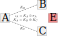
\includegraphics[draft=false, width=0.6\linewidth]{qss/qss_honest_recipients}
\caption{\label{fig:qss_honest_recipients} Alice distributes her secret $\sigma_A$ to Bob and Charlie who are assumed honest. Dishonest Eve will try to attack the protocol and gain information about $\sigma_A$. Gray: honest. Red: dishonest. See Fig.~\ref{fig:qss_structure} for further information.}
\end{figure}


The starting point for our security analysis is the following Devetak-Winter bound \cite{Devetak2004} for the asymptotic key rate under collective attack, Fig.~\ref{fig:types_of_attack_collective}:

%\MT{should I motivate why this bound is helpful for us?}

\begin{equation}\label{eqn:qss_dw_eve}
\kappa_{\text{Eve}} \ge \text{I}\left(X_A : X_B, X_C\right) - \chi\left(X_A : \mathbb{E}\right).
\end{equation}

\noindent This equation describes the key rate in terms of the difference between the mutual information, $\text{I}$, shared between Alice and a Bob-Charlie collaboration, and the Holevo information $\chi$ between Eve's quantum system $\mathbb{E}$ and Alice. %\footnote{It is perhaps unsurprising that Eq.~\ref{eqn:qss_dw_eve} should be our starting point given the noted similarities between QSS and QKD.}
The $X_A = \mathcal{F}\left(A_B, A_C\right)$ is Alice's variable based on her heterodyne measurement outcomes.

We would like to calculate the lower bound for key rate given by Eq.~\ref{eqn:qss_dw_eve} and so we will consider each term, and demonstrate how they may be calculated in our protocol.



\subsection{Mutual information}

Using Eq.~\ref{eqn:intro_mutual_information}, the mutual information $\text{I}$ may be written as 
\begin{equation}\label{eqn:qss_deriv_1}
\text{I}\left(X_A : X_B, X_C\right) = \text{H}\left(X_B, X_C\right) - \text{H} \left(X_B, X_C \given X_A\right),
\end{equation}
where the first term on the right hand side is the joint Shannon entropy of $X_B$ and $X_C$, and the second term is the conditional Shannon entropy of $X_B, X_C$ given $X_A$, Sec.~\ref{sec:intro_shannon_entropy}. Intuitively, this second term encodes the uncertainty one has about which $X_B, X_C$ were chosen, once Alice has formed $X_A$. The first term encodes the \emph{a priori} entropy about Bob and Charlie's choice of sent coherent states, and is purely a function of their sending probabilities.

The joint Shannon entropy may be written
\begin{equation}\label{eqn:qss_deriv_2}
\text{H}\left(X_B, X_C\right) = \sum_{X_B=\phi_B, X_C=\phi_C} - \text{P}\left(\phi_B, \phi_C\right) \log \text{P}\left(\phi_B, \phi_C\right),
\end{equation}
where $\phi_B, \phi_C$ are individual instances of variables $X_B, X_C$. We take $\phi_B, \phi_C$ as phase elements of the QPSK alphabet, is easy to generalize to larger $N$PSK alphabets if desired. Since $\phi_B, \phi_C$ are taken to be independently and randomly chosen, each with probability\footnote{We relax this in Ch.~\ref{chapter:aqc}.} $1/4$, we see that the joint probability
\begin{equation}\label{eqn:qss_deriv_3}
\text{P}\left(\phi_B, \phi_C\right) = \text{P}\left(\phi_B\right)\times \text{P}\left(\phi_C\right) = \frac{1}{16},
\end{equation}
and so $\text{H}\left(X_B, X_C\right) = 4$. %TODO: check this

Expanding the conditional entropy in terms of particular outcomes for $X_A$, via Eq.~\ref{eqn:intro_conditional_entropy_expansion}%\cite{Wilde2013}, 
, we reach

\begin{equation}\label{eqn:qss_deriv_4}
\text{H}\left(X_B, X_C \given X_A\right) = \int\limits_{a \in \mathbb{C}} \Diff2 a \; \text{P}\left(X_A = a\right) \text{H}\left(X_B, X_C \given X_A = a\right).
\end{equation}
Each term in Eq.~\ref{eqn:qss_deriv_4} can be calculated once function $\mathcal{F}$ is known. The conditional entropy $\text{H}\left(X_B, X_C \given X_A = a\right)$ expands as 

\begin{align}
\text{H}\left(X_B, X_C \given X_A=a\right) = - \sum_{\phi_B, \phi_C} \;  &\text{P}\left(X_B=\phi_B, X_C=\phi_C \given X_A=a\right) \times \notag \\
%
&\log \text{P}\left(X_B=b, X_C=c \given X_A=a\right) \label{eqn:qss_deriv_4_1}
\end{align}

\noindent and so all that remains to calculate are the probabilities 
\begin{align}
\label{eqn:qss_prob1} \text{P}\left(X_A=a\right) \qq{and} \\
\label{eqn:qss_prob2} \text{P}\left(X_B=\phi_B, X_C=\phi_C \given X_A=a\right)
\end{align}
once $\mathcal{F}$ is known.


\subsubsection{Function $\mathcal{F}$}


We have no requirement that the function $\mathcal{F}$ should be injective. This implies, for example, that $\text{S}\left(\rho_{\left.\mathbb{E} \given A_B, A_C\right.}\right) \ne \text{S}\left(\rho_{\left. \mathbb{E} \given X_A\right.}\right)$, i.e. the entropy of Eve's quantum state conditioned on Alice's heterodyne outcomes $A_B, A_C$ is not equal to the entropy of Eve's quantum state conditioned on Alice's variable $X_A$. So, we must carefully consider the action of $\mathcal{F}$ early on in our analysis. 

To be concrete, in what follows we assume that $F$ is linear,
\begin{equation}\label{eqn:qss_F_linear}
\mathcal{F}\left(x, y\right) := g x + h y \qq{with} g, h \in \mathbb{R}\setminus \left\{0\right\},
\end{equation} 
which will enable us to make some predictions about the performance of the protocol. Although we make no claims about the optimality of this choice of $\mathcal{F}$, Alice is free to optimize the key rate over $g, h$.

%, and we will make it clear when we have done so. In Sec.~\ref{appendix:qss_moreF} we consider some alternative forms for $\mathcal{F}$.





\subsubsection{Expanding classical probabilities}

Applying Bayes' formula Eq.~\ref{eqn:intro_bayes} to probability Eq.~\ref{eqn:qss_prob2} we see that
\begin{align}
\text{P}\left(X_B=\phi_B, X_C=\phi_C \given X_A=a\right) = \text{P}&\left(X_A=a \given X_B=\phi_B, X_C=\phi_C\right) \notag \\
&\times \frac{\text{P}\left(X_B=\phi_B, X_C=\phi_C\right)}{\text{P}\left(X_A=a\right)}.
\end{align}


\noindent Now, we can access $\text{P}\left(X_A=a \given X_B=\phi_B, X_C=\phi_C\right)$. 
%by modelling the effects of the channel on quantum states distributed by Bob and Charlie. 
We take
\begin{equation}\label{eqn:qss_deriv_5}
X_A = \mathcal{F}\left(A_B, A_C\right) = g A_B + h A_C,
\end{equation}
as in Eq.~\ref{eqn:qss_F_linear}, and so we rearrange:
\begin{equation}
A_C = \frac{X_A - g A_B}{h}.
\end{equation}

\noindent Since our $\mathcal{F}$ is not injective %(there are multiple $A_B, A_C$ which will give the same $X_A$)
we must average over all of the possible ways to reach a given $X_A$. Therefore, once $X_A, g$ and $h$ are fixed, the choice of $A_B, A_C$ reduces to a one-variable problem. So

\begin{equation}\label{eqn:qss_deriv_5_1}
\text{P}\left(X_A \given X_B=\phi_B, X_C=\phi_C\right) = \int\limits_{A_B \in \mathbb{C}} \Diff2 A_B \; \text{P}\left(A_B , \frac{X_A - g A_B}{h} \given X_B=\phi_B, X_C=\phi_C\right)
\end{equation}
which may be calculated once we know how the channel acts on input states\footnote{Note that an analogous expression would be reached by rearranging Eq.~\ref{eqn:qss_deriv_5} as $A_B = \left(X_A - h A_C\right)/g$, but it will make no difference to the resulting quantities which we derive from Eq.~\ref{eqn:qss_deriv_5_1}}.

Assuming that the two channels, one from Charlie$\rightarrow$Alice and one from Bob$\rightarrow$Alice, are independent\footnote{We shall see later what this means for their combined action on an input quantum state} from each other allows us to write
\begin{equation}\label{eqn:qss_deriv_6}
\text{P}\left(A_B, A_C \given X_b=\phi_B, X_C=\phi_C\right) = \text{P}\left(A_B \given X_B=\phi_B\right) \times \text{P}\left(A_C \given X_C=\phi_C\right)
\end{equation}
for the probabilities that Alice's heterodyne measurement outcomes are $A_B, A_C$, given that coherent states with phases $\phi_B, \phi_C$ are sent.

Let us assume for now that each channel is noiseless but lossy. The probability that Alice measures a particular heterodyne outcome $a = \qout + i \pout$ when a coherent state of complex amplitude $\beta$ is sent through a lossy channel, transmittivity $T$, is  %where do I actually derive this? I should put it in one place and then refer to it a bunch
\begin{equation}\label{eqn:qss_channel_classical_prob}
\text{P}\left(a \given \beta, T\right) = \frac{1}{\pi}\exp\left( - \left| a - \sqrt{T}\beta \right|^2\right)
\end{equation}
which we have used previously in Ch.~\ref{chapter:qds}. The required changes to include thermal noise of the channel can be readily made, Appendix.~\ref{appendix:noisy_perr}.

The integral in Eq.~\ref{eqn:qss_deriv_5_1} may now be calculated analytically to reach 
\begin{align}\label{eqn:qss_deriv_7}
\text{P}\left(X_A \given X_B=\phi_B, X_C=\phi_C\right) = \frac{1}{\pi} \frac{1}{g^2 + h^2} &\exp \left( - \frac{\left[\phi_B^R g \sqrt{T_B} + \phi_C^R h \sqrt{T_C} - X_A^R \right]^2}{g^2 + h^2}\right) \notag \\
%
&\times \exp \left( - \frac{\left[\phi_B^I g \sqrt{T_B} + \phi_C^I h \sqrt{T_C} - X_A^I \right]^2}{g^2 + h^2} \right).
\end{align}
Here $\phi_B, \phi_C$ are Bob and Charlie's coherent state amplitudes, $X_A$ is Alice's final variable after applying $\mathcal{F}$ (Eq.~\ref{eqn:qss_F_linear}) to her heterodyne outcomes, $T_B, T_C$ are the transmittivities of the Bob$\rightarrow$Alice channel and Charlie$\rightarrow$Alice channel, respectively, and a superscript $R\left(I\right)$ denotes the real (imaginary) part of the corresponding quantity. %\MT{I probably don't need to say much about how this integration is actually done, since it should be obvious.} 
The probability $\text{P}\left(X_A=a\right)$ Eq.~\ref{eqn:qss_prob1} may now be found by summing over Eq.~\ref{eqn:qss_deriv_7}:

\begin{equation}\label{eqn:qss_deriv_pxa}
\text{P}\left(X_A\right) = \sum_{\phi_B, \phi_C} \text{P}\left(X_A \given X_B=\phi_B, X_C=\phi_C\right).
\end{equation}


Finally, the mutual information Eq.~\ref{eqn:qss_deriv_1} may be calculated. We perform the integration over $X_A$ in Eq.~\ref{eqn:qss_deriv_4} numerically and display the mutual information $I$ in Fig.~\ref{fig:qss_mutual_information}.


\subsection{Holevo information}

We will now detail how the Holevo information term, $\chi$ in Eq.~\ref{eqn:qss_dw_eve}, may be calculated. In doing so we will point to areas where future work might strengthen the security analysis to consider wider classes of attack. This should illuminate the contexts to which our security proof may be applied. In this section we consider a dishonest Eve performing attack BS$0$, as detailed above in Sec.~\ref{sec:qds_bs0}, though the analysis follows readily for the other attacks described in Sec.~\ref{sec:qds_attack_analysis}. %We will then compare the strength of attacks BS$0$, BS$1$, BS$2$ and EC. % and more general attacks will be considered later.

Bob and Charlie prepare a state from the QPSK alphabet, and each state is chosen randomly and with equal probability. Before the channel, Bob and Charlie hold the joint state
\begin{equation}
\rho_{\text{before}} = \rho_B \otimes \rho_C
\end{equation}
with
\begin{equation}\label{eqn:qss_initial_states}
\rho_B = \frac{1}{4} \sum_{k=0}^3 \dyad{\beta_k}_B \qq{and} \rho_C = \frac{1}{4} \sum_{k^\prime = 0}^3 \dyad{\gamma_{k^\prime}}_C
\end{equation}
where $\beta, \gamma$ are the amplitudes of Bob's and Charlie's coherent state alphabets.

We assume that the channel acts separately on each mode, and that modes $\rho_B$, $\rho_C$ undergo independent evolution. In other words, we assume that the channel has the following structure:
\begin{equation}\label{eqn:qss_channel}
\Phi\left[\rho\right] = \Phi_B\left[\rho\right] \otimes \Phi_C\left[\rho\right]
\end{equation}
where $\Phi_{B, C}$ denote the lossy channels described by attack BS$0$, Sec.~\ref{sec:qds_bs0}, and the subscript $B, C$ denotes which mode of $\rho_{\text{before}}$ each channel acts on. The total channel $\Phi$ preserves the tensor-product structure of the input state.

Physically $\Phi$ corresponds to the case where Eve performs separate beamsplitter attacks on each channel and retains two output modes $\mathbb{E}_{B, C}$, Fig.~\ref{fig:qss_bs0_attack}.

\begin{figure}[htp]
\captionsetup{width=0.8\linewidth}
\centering
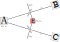
\includegraphics[draft=false, width=\linewidth]{qss/qss_bs0}
\caption{\label{fig:qss_bs0_attack} We model the channel $\Phi$ as two independent beamsplitter attacks of type BS$0$, Sec.~\ref{sec:qds_bs0}. This preserves the tensor-product structure of $\rho_{\text{before}}$.}
\end{figure}


The total state after the channel becomes
\begin{equation}
\rho_{\text{after}} = \rho_{\mathbb{A}_B, \mathbb{E}_B} \otimes \rho_{\mathbb{A}_C, \mathbb{E}_C},
\end{equation}
with $\mathbb{A}_{B, C}$ denoting Alice's two modes and where
\begin{equation}
\rho_{\mathbb{A}_B, \mathbb{E}_B} = \frac{1}{4} \sum_{k=0}^3 \dyad{\sqrt{T_B} \beta_k}_{\mathbb{A}_B} \otimes \dyad{\sqrt{1-T_B} \beta_k}_{\mathbb{E}_B},
\end{equation}
and similarly for $\rho_{\mathbb{A}_C, \mathbb{E}_C}$. Now, Alice heterodynes and measures $A_B$ from $\rho_{\mathbb{A}_B, \mathbb{E}_B}$ and $A_C$ from $\rho_{\mathbb{A}_C, \mathbb{E}_C}$. Eve's total state conditioned on these outcomes becomes 
\begin{equation}\label{eqn:qss_eve_conditional}
\rho_{\left.\mathbb{E} \given A_B, A_C\right.} = \rho_{\left.\mathbb{E}_B \given A_B\right.} \otimes \rho_{\left. \mathbb{E}_C \given A_C\right.},
\end{equation}
with
\begin{equation}
\rho_{\left.\mathbb{E}_B \given A_B\right.} = \frac{1}{4 \pi} \sum_{k=0}^3 \text{P}_B\left(A_B \given \beta_k, T_B\right) \dyad{\sqrt{1-T_B} \beta_k}_{\mathbb{E}_B},
\end{equation}
and similarly for $\rho_{\left.\mathbb{E}_C \given A_C\right.}$. The probability $\text{P}_B\left(A_B \given \beta_k, T_B\right)$ is calculated analogously to Eq.~\ref{eqn:qss_channel_classical_prob}, and similarly for $A_C$.

To proceed, we take $X_A = g A_B + h A_C$ as usual, with $g, h$ fixed, and write $A_C = \left(X_A - g A_B\right)/h$. Therefore the state $\rho_{\left.\mathbb{E} \given A_B, A_C\right.}$, Eq.~\ref{eqn:qss_eve_conditional}, becomes

\begin{align}\label{eqn:qss_deriv_8}
&\rho_{\left. \mathbb{E} \given X_A, A_B\right.} = \frac{1}{16 \pi^2} \sum_{k, k^\prime = 0}^3 \text{P}_B\left(A_B \given \beta_k, T_B\right) \text{P}_C\left(\frac{X_A - g A_B}{h} \given \gamma_{k^\prime}, T_C\right) \notag \\
%
&\times \dyad{\sqrt{1-T_B} \beta_k}_{\mathbb{E}_B} \otimes \dyad{\sqrt{1-T_C}\gamma_{k^\prime}}_{\mathbb{E}_C}.
\end{align}

\noindent Once again, since Alice's function $\mathcal{F}$ is in general not injective, we must mix over outcomes $A_B, A_C$ in order to find Eve's state $\rho_{\left.\mathbb{E} \given X_A\right.}$:

\begin{equation}\label{eqn:qss_aposteriori_state}
\rho_{\left.\mathbb{E} \given X_A\right.} = \int\limits_{A_B \in \mathbb{C}} \Diff2 A_B \; \text{P}\left(A_B\right) \rho_{\left.\mathbb{E} \given X_A, A_B\right.}.
\end{equation}

\noindent Mixing over $X_A$ we finally reach

\begin{equation}\label{eqn:qss_apriori_state}
\rho_{\mathbb{E}} = \int\limits_{X_A \in \mathbb{C}} \Diff2 X_A \; \text{P}\left(X_A\right) \rho_{\left.\mathbb{E}\given X_A\right.}.
\end{equation}

\noindent We may identity Eq.~\ref{eqn:qss_aposteriori_state} as Eve's \emph{a prosteriori} state and Eq.~\ref{eqn:qss_apriori_state} as Eve's \emph{a priori} state and so Eve's Holevo information is given by the usual formula Eq.~\ref{intro_stuff}:

\begin{equation}\label{eqn:qss_holevo}
\chi = \text{S}\left(\rho_\mathbb{E}\right) - \int\limits_{X_A \in \mathbb{C}} \Diff2 X_A \; \text{P}\left(X_A\right) \text{S}\left(\rho_{\left.\mathbb{E} \given X_A\right.}\right).
\end{equation}

We note that we can no longer simplify the second term in Eq.~\ref{eqn:qss_holevo}, like we did in Sec.~\ref{sec:qds_attack_analysis}, for example, since in general the entropy of each state depends on $X_A$. We perform the integration in Eq.~\ref{eqn:qss_holevo} numerically, and display the output Holevo information in Fig.~\ref{fig:qss_holevo_information}.


\section{Security against a dishonest player}\label{sec:qss_dishonest_recipient}
%\MT{Talk about guarding against a dishonest Bob/Charlie.}
Of course, if Alice only had to guard against an external Eve, and both Bob and Charlie could be assumed honest, then the QSS task becomes much easier. She could, for example, simply send the same information to each recipient. Or send her secret just to the recipient she is interested in, with no need to ``split'' it or share it. The task of secret sharing, however, assumes dishonest recipients. In this section we will adapt the analysis of Sec.~\ref{sec:qss_honest_recipients} to this case. Our method will be to take the final key rate as the minimum of key rates under dishonest Bob and dishonest Charlie, which therefore secures against both possibilities \cite{Kogias2017, Grice2019}. %TODO: make sure I can talk about this for the viva.

\subsection{Dishonest Bob}
Let us translate the analysis from Sec.~\ref{sec:qss_honest_recipients} to the case where either Bob or Charlie is dishonest, but Alice does not know which one, Fig.~\ref{fig:qss_structure}. Including a dishonest recipient in the above security proof requires us to re-calculate several quantities. For concreteness we will first assume that Bob is dishonest and Charlie is honest, Fig.~\ref{fig:qss_dishonest_Bob}, and we will allow Bob to collaborate with Eve. Later we will discuss how to account for the fact that we do not know \emph{which} player is dishonest.

\begin{figure}[htp]
\captionsetup{width=0.8\linewidth}
\centering
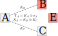
\includegraphics[draft=false, width=0.6\linewidth]{qss/qss_dishonest_Bob}
\caption{\label{fig:qss_dishonest_Bob} A dishonest Bob gains an advantage since he knows which coherent state he chose to send to Alice. He may additionally choose to collaborate with Eve in order to gain information about Alice's measurement on Charlie's state. c.f. Fig.~\ref{fig:qss_structure}.}
\end{figure}

The main effect of permitting dishonesty from Bob is that he knows precisely which coherent states he sent to Alice. This reduces his uncertainty about Alice's variable $X_A$. Bob might also wait and see which coherent state was sent by Charlie before choosing his own, in order to preference a certain outcome $X_A$, but the advantage that this might give may be reduced by assuming that $\mathcal{F}$, $g$ and $h$ are not disclosed by Alice at the start of the protocol. We will discuss this further in Sec.~\ref{sec:qss_outlook}. We will additionally assume that Bob sends states only from the QPSK alphabet, though in principle this could be relaxed in future work.

Since Bob knows which coherent state he sent, we must re-calculate several expressions from Sec.~\ref{sec:qss_honest_recipients}. The main change is that we no longer mix over Bob's alphabet. The quantities which this influences are $\text{P}\left(X_A=a\right)$ and $\text{H}\left(X_B, X_C \given X_A=a\right)$, which now become

\begin{equation}
\text{P}\left(X_A=a\right) = \sum_{c} \text{P}\left(X_A \given X_b=b, X_C=c\right),
\end{equation}

\noindent and

\begin{align}
\text{H}\left(X_B, X_C \given X_A=a\right) = - \sum_{c} \text{P}&\left(X_B=b, X_C=c \given X_A=a\right) \times \notag \\
&\log \text{P}\left(X_B=b, X_C=c \given X_A=a\right).
\end{align}

\noindent The mutual information may now be calculated as in the previous section. 

The Holevo information is also calculated analogously to the previous section, the key change being that Eve's state conditioned on $X_A, A_B$, Eq.~\ref{eqn:qss_deriv_8}, is now given by
\begin{align}\label{eqn:qss_deriv_9}
\rho_{\left.\mathbb{E} \given X_A, A_B\right.} &= \frac{1}{4 \pi^2} \sum_{k^\prime=0}^3 \text{P}_B\left(A_B \given \beta_k, T_B\right) \text{P}_C\left(\frac{X_A - g A_B}{h} \given \gamma_{k^\prime}, T_C\right) \notag \\
%
&\dyad{\sqrt{1-T_B} \beta_k}_{\mathbb{E}_B} \otimes \dyad{\sqrt{1-T_C}\gamma_{k^\prime}}_{\mathbb{E}_C}
\end{align}
and the \emph{a posteriori} and \emph{a priori} states calculated by integrating Eq.~\ref{eqn:qss_deriv_9} identically to Eqs.~\ref{eqn:qss_aposteriori_state},~\ref{eqn:qss_apriori_state}.

Since we no longer mix over Bob's coherent state $\beta_k$, the mutual information $\text{I}$ and Holevo information $\chi$ have themselves become functions of $\beta_k$. In this chapter we assume that each state in the QPSK alphabet is equally likely and has equal magnitude and so both $\text{I}$ and $\chi$ will be identical for each of Bob's alphabet states. We will relax this in Chapter~\ref{chapter:aqc}.


The final key rate is now
\begin{equation}\label{eqn:qss_keyrate_dishonest_Bob}
\kappa_{\text{Eve, Bob}} = \text{I}\left(X_A : X_B, X_C\right) - \chi\left(X_A : \mathbb{E} \mathbb{B}\right)
\end{equation}
with mutual information and Holevo information terms calculated as described above. In using Eq.~\ref{eqn:qss_keyrate_dishonest_Bob} we are treating Bob as a dishonest eavesdropper who collaborates with Eve. This key rate formula thus provides security against general collective eavesdropping strategies, provided the mutual information and Holevo information terms can be bounded. In this Chapter we will allow the same range of attacks as in Ch.~\ref{chapter:qds}. We discuss additional attack strategies unique to our QSS protocol in Sec.~\ref{sec:qss_outlook}. 


%\MT{Make some graphs of things with dishonest Bob}


\subsection{Dishonest Bob or Dishonest Charlie}
If Alice is certain that Bob is the dishonest player then she has no need for a secret sharing scheme. Equivalently, she can set $g=0$ in her function $\mathcal{F}$. If she is correct about Bob's dishonestly, then she has successfully prevented him from gaining any information about her secret. However, if Alice turns out to be wrong and it is Charlie who is the dishonest player then she has accidentally given Charlie the secret! It is precisely this uncertainty about which player is dishonest which makes a QSS scheme necessary.

In order to take into account this uncertainty over which player is dishonest, Fig.~\ref{fig:qss_structure}, we proceed as in the recent QSS works Refs.~\cite{Kogias2017, Grice2019} and calculate the minimum over all possible dishonest configurations. That is, we take

\begin{equation}\label{eqn:qss_key_rate_min}
\kappa \ge \min \left\{\kappa_{\text{Eve, Bob}}, \kappa_{\text{Eve, Charlie}}\right\}
\end{equation}
where $\kappa_{\text{Eve, Charlie}}$ is calculated analogously to Eq.~\ref{eqn:qss_keyrate_dishonest_Bob}. This expression makes explicit the close links between QSS and QKD, as explored further in Refs.~\cite{Kogias2017, Grice2019}. The work by Grice \cite{Grice2019} generalizes this expression to $N$ players, and directly comments that their setup can perform both QSS and $2$-party QKD with rate calculated analogously.


\section{Protocol performance}\label{sec:qss_performance}


We plot the mutual information (Eq.~\ref{eqn:qss_deriv_1}) in Fig.~\ref{fig:qss_mutual_information}, taking honest recipients in (a) and dishonest recipients in (b). Coherent state amplitude $\alpha$ and channel transmission $T$ are varied. We here take Bob and Charlie's states as having equal amplitudes and channel transmissions, but in principle they can vary independently from one another. Unless $T=0$, the mutual information between Alice and Bob-Charlie always increases with $\alpha$ as the states at Alice become increasingly distinguishable. The mutual information with honest recipients is bounded by $4$, while in the case of dishonest recipients it is bounded by $2$. 

\begin{figure}[htp]
\captionsetup{width=0.8\linewidth}
\centering
	\begin{subfigure}{0.49\linewidth}
	\centering
	\includegraphics[draft=false, width=\linewidth]{qss/mutinf_honest_symmetric_a_T}
	\caption{}
	\end{subfigure}
	\begin{subfigure}{0.49\linewidth}
	\centering
	\includegraphics[draft=false, width=\linewidth]{qss/mutinf_dishonest_symmetric_a_T_and_honest}
	\caption{}
	\end{subfigure}
\caption{\label{fig:qss_mutual_information} Mutual information Eq.~\ref{eqn:qss_deriv_1} as it varies with coherent state amplitude $\alpha$ and channel transmission $T$. (a) Honest recipients. (b) Orange: dishonest recipients. Blue, clear: honest recipients, same surface as (a). In both figures we have taken linear $\mathcal{F}$, with parameters $g = h = 0.5$.}
\end{figure}

The Holevo information $\chi$ under identical conditions to Fig.~\ref{fig:qss_mutual_information} is plotted in Fig.~\ref{fig:qss_holevo_information}. We see that there is a clear maximum of $\chi$ at $T = 0.5$, which is when dishonest parties have maximum fidelity to Alice's received state. Our QSS protocol leverages the power of cryptographic protocols constructed in the reverse-reconciliation regime. As $T < 0.5$, even though Eve receives a greater share of the sent state than Alice\footnote{This would be fatal for direct-reconciliation cryptography.}, the overlap between Eve's and Alice's states begins to decrease as $T$ decreases, meaning $\chi$ also decreases.

Curiously, Fig.~\ref{fig:qss_holevo_information}b demonstrates a reduction in the Holevo information when Bob or Charlie is dishonest. Since Holevo information is directly related to the efficacy of an attack, this might suggest that dishonesty gives no advantage, and even makes things worse. We note however that the mutual information is also reduced in this case, and a consideration of the key rate in Fig.~\ref{fig:qss_keyrate} demonstrates that such dishonesty of Bob or Charlie does indeed yield a reduction in the key rate $\kappa$. %The reduction in $\chi$ is explained by noting that there is one fewer channel being attacked, and that the Holevo information represents the amount of information gained via an attack. %TODO: make sure I can talk about this for the viva.

\begin{figure}[htp]
\captionsetup{width=0.8\linewidth}
\centering
	\begin{subfigure}{0.49\linewidth}
	\centering
	\includegraphics[draft=false, width=\linewidth]{qss/holevo_honest_symmetric_a_T}
	\caption{}	
	\end{subfigure}
	\begin{subfigure}{0.49\linewidth}
	\centering
	\includegraphics[width=\linewidth, draft=false]{qss/holevo_dishonest_symmetric_a_T_and_honest}
	\caption{}	
	\end{subfigure}
\caption{\label{fig:qss_holevo_information} Holevo information Eq.~\ref{eqn:qss_holevo} as it varies with coherent state amplitude $\alpha$ and channel transmission $T$. (a) Honest recipients. (b) Orange: dishonest recipients. Blue, clear: honest recipients, same surface as (a). In both figures we have taken linear $\mathcal{F}$, with parameters $g = h = 0.5$.}
\end{figure}

The key rate $\kappa$ is plotted in Fig.~\ref{fig:qss_keyrate}. Comparing Fig.~\ref{fig:qss_keyrate}(a) and (b), we see that in all cases the presence of dishonesty in Bob or Charlie causes a reduction in the obtained key rate. Each figure takes Bob and Charlie to have the same coherent state amplitude $\alpha$ and channel transmission $T$. At the loss levels considered here, $\alpha=0.8$ yields larger $\kappa$, but for larger losses (not shown) $\alpha=0.5$ performs better. Indeed, the best $\alpha$ reduces as the loss level increases. We found a similar result for our QDS protocol, Fig.~\ref{fig:qds_gsec_croal}.

We see that a symmetric choice $g = h = 0.5$ is clearly optimal when both Bob and Charlie are honest (green and blue lines in (a) outperform red and orange), while the best choice of $g, h$ in (b) depends on which player is assumed dishonest. For example, assuming that Bob is dishonest gives much larger $\kappa$ for $g=0.2$, $h=0.8$ (orange in (b)) than for $g = h = 0.5$ (blue in (b)). By lowering $g$ we are effectively reducing the amount of information which Bob has access to, and his knowledge of which state was sent matters less and less. Conversely, the choice $g=0.2$, $h=0.8$ causes a large reduction in $\kappa$ when Charlie is dishonest. Since the final key rate $\kappa$ is a minimum over these two key rates, Eq.~\ref{eqn:qss_key_rate_min}, we see that when either party can be dishonest the optimal choice should be the symmetric choice $g=h$. It would however be interesting to see how optimal parameter choices vary with the number of players and potential adversarial collaborations.



\begin{figure}[htp]
\captionsetup{width=0.8\linewidth}
\centering
	\begin{subfigure}{0.49\linewidth}
	\centering
	\includegraphics[draft=false, width=\linewidth]{qss/keyrate_honest_1}
	\caption{}
	\end{subfigure}
	\begin{subfigure}{0.49\linewidth}
	\centering
	\includegraphics[draft=false, width=\linewidth]{qss/keyrate_dishonest_1}
	\caption{}
	\end{subfigure}
\caption{\label{fig:qss_keyrate} QSS key rates varying with dB loss. Bob and Charlie experience the same loss, and begin with the same input alphabet amplitude. (a) Honest Bob and Charlie. (b) Dishonest Bob and Charlie. (a) and (b) - blue: $\alpha=0.5$, $g=h=0.5$; green: $\alpha = 0.8$, $g = h = 0.5$; orange: $\alpha = 0.5$; $g = 0.2$, $h=0.8$ Bob dishonest; red: $\alpha = 0.5$; $g=0.2$, $h=0.8$ Charlie dishonest.}
\end{figure}


Allowing for Bob and Charlie to experience different loss levels, or use different input alphabet amplitudes, we plot the resultant key rates in Fig.~\ref{fig:qss_keyrate_asymmetric}. In (a) we let $g=0.2$, $h=0.8$ (blue, green) and $g=0.3$, $h=0.7$ (orange, red) and vary the channel loss of Bob, while Charlie's is fixed at $-1.5$~dB. Bob is assumed dishonest. We see that the loss variation in the player who contributes little to the key, in this case Bob as $g < h$, leads to only small changes in the resultant $\kappa$. However, when Charlie's loss varies and Bob's remains constant, for equivalent parameters, we see (b) large variations in $\kappa$. Black lines denote $g=h=0.5$ with only Bob's loss (a) or Charlie's loss (b) varying. Gray, dashed lines denote $g=h=0.5$ when Bob and Charlie's losses vary equally. We see from this Figure~\ref{fig:qss_keyrate_asymmetric} that when $g \ne h$, the channel parameters of the player who contributes most to the key (Bob if $g < h$ or Charlie if $h < g$) make the most significant impact. Interestingly, for the symmetric case $g=h$, which we have already noted is the optimal choice, it is the largest amount of loss which controls $\kappa$. Little is to be gained by having one high quality channel if the other one is poor. 


\begin{figure}[htp]
\centering
	\begin{subfigure}{0.49\linewidth}
	\centering
	\includegraphics[width=\linewidth, draft=false]{qss/asymmetric_keyrates_1}
	\caption{}
	\end{subfigure}
	\begin{subfigure}{0.49\linewidth}
	\centering
	\includegraphics[width=\linewidth, draft=false]{qss/asymmetric_keyrates_2}
	\caption{}
	\end{subfigure}
\caption{\label{fig:qss_keyrate_asymmetric} QSS key rates varying dB loss asymmetrically. (a) Bob's loss varies, while Charlie's remains at $-1.5$~dB. (b) Charlie's loss varies, while Bob's remains at $T=0.7$. (a)-(b): We have taken $g = 0.2, h=0.8$ (blue, green); $g=0.3, h=0.7$ (orange, red). Blue and orange lines: both Bob and Charlie are honest. Green and red lines: Bob is dishonest. Varying the loss of the dishonest player (a) results in negligible variation of $\kappa$, while varying loss of honest player (b) results in large variation. Black: $g=h=0.5$ varying loss of honest player. Gray, dashed: $g=h=0.5$ varying loss of honest and dishonest player equally.}
\end{figure}






\section{Outlook}\label{sec:qss_outlook}
We have introduced and demonstrated a fully continuous-variables protocol which performs the QSS task. Our protocol relies only on distribution of QPSK coherent states and phase measurement via heterodyne detection. Our protocol is proven secure against collective attacks for which the Holevo information $\chi$ may be bounded, and we have demonstrated how this may be estimated under beamsplitter attacks (Sec.~\ref{sec:qds_attack_analysis}). In principle our analysis may readily include entangling cloner attacks, as we did in Ch.~\ref{chapter:qds} for the QDS protocol, but as we shall see later in Ch.~\ref{chapter:aqc} the QSS protocol is not very robust to channel excess noise. This might have been expected, as QKD protocols with similar resources \cite{Papanastasiou2018, Zhao2009} allow only very small amounts of noise in the reverse-reconciliation configuration before a secure key cannot be formed. 

We will revisit this QSS protocol in Chapter~\ref{chapter:aqc} where we shall investigate its experimental implementation alongside other cryptographic schemes with identical hardware requirements, and we shall see in particular that this QSS protocol requires fewer quantum resources than pairwise-QKD followed by a classical unconditionally secure secret sharing scheme, Sec.
\ref{sec:aqc_performance}.

The classical post-processing of the above protocol is inherently very similar to Ref.~\cite{Kogias2017}, in which a secret key is generated between Alice and a shared Bob-Charlie degree of freedom via incompatible homodyne measurements on a tripartite entangled state. We have several reasons to expect that our protocol will be secure against a more restricted set of attacks, but over a wider range of channel parameters.  Firstly unlike Ref.~\cite{Kogias2017} which relies in generation and distribution of large multipartite entangled states, our scheme has more modest quantum requirements which are easier to generate and manipulate, and which are much more robust to channel loss and channel noise than a large entangled state. Quantum cryptography (QKD, QDS) using continuous-variables typically operates over metropolitan distances of tens of kilometers, and so we might reasonably expect similar performance of our QSS protocol. Performance of our protocol over a realistic fiber channel is analysed in Chapter~\ref{chapter:aqc}. Secondly, the protocol from Ref.~\cite{Kogias2017} takes a form analogous to direct-reconciliation (DR) QKD, while ours is analogous to reverse-reconciliation (RR) QKD. RR QKD is known \cite{Grosshans2002, Grosshans2003, Laudenbach2017} to be much more resilient to loss and noise than DR QKD without modifications \cite{Silberhorn2002}.

Ref.~\cite{Kogias2017} has potentially dishonest players Bob and Charlie performing homodyne measurements on incompatible observables (i.e. switching between $q$ and $p$ quadratures). No assumptions are made about the measurement devices used and they are each treated as a "black-box". Security there comes inherently because of a Heisenberg-type relation between incompatible observables, and the security proof relies on an Entropic Uncertainty Relation which has had success in many parts of quantum cryptography \cite{Furrer2012, Furrer2017}. However, since we desire to use heterodyne detection we are forced to adopt a different approach and explicitly model the states' evolution and measurement during the protocol. We note that this matches the current state-of-the-art of QPSK-based QKD \cite{Papanastasiou2018}, but should be improved in future work. One approach might be to use an Entropic Uncertainty Relation designed with heterodyne detection in mind \cite{DePalma2017i, DePalma2017}, but our preliminary analysis has been pessimistic.

We have assumed that a dishonest Bob or Charlie still sends a state from the QPSK alphabet. It is yet unclear whether they could gain an advantage by sending something exotic and potentially highly entangled, perhaps in order to force Alice to reach a certain key $X_A$. This should be explored and potentially relaxed in future work. One solution might be for Alice to wait until after Distribution to declare her choice of $\mathcal{F}$ and its parameters, which in the worst-case scenario should lead to a final security bound based on assumptions about the power of existing quantum memory devices. This approach was used in recent proofs for security of quantum oblivious transfer \cite{Furrer2017, Broadbent2015}. We anticipate also that applying methods from quantum bit commitment \cite{Broadbent2015} might prove fruitful here, since bit commitment also allows for possible dishonest distribution of the quantum state from an untrusted player. Finally, we note that our assumption that the channel between Alice and Bob-Charlie takes a tensor-product structure, Eq.~\ref{eqn:qss_channel}, Fig.~\ref{fig:qss_bs0_attack} should be relaxed. %A potential strategy of a dishonest player could be to exploit properties of a general channel which maps a two-mode input state to a two-mode output state at Alice, potentially allowing a dishonest player many output ancilla modes correlated with Alice. Such a strategy will be restricted by the conditions that the reduced state of an honest player should be a coherent state (with noise). Similarly it will require that Alice's measurement outcomes don't look ``too errant'', though this should be quantified.





